% --- INICIO CÓDIGO PARA anexos.tex ---
% Este archivo contiene el código LaTeX para los anexos del documento principal.
% Se incluye en main.tex usando % --- INICIO CÓDIGO PARA anexos.tex ---
% Este archivo contiene el código LaTeX para los anexos del documento principal.
% Se incluye en main.tex usando % --- INICIO CÓDIGO PARA anexos.tex ---
% Este archivo contiene el código LaTeX para los anexos del documento principal.
% Se incluye en main.tex usando % --- INICIO CÓDIGO PARA anexos.tex ---
% Este archivo contiene el código LaTeX para los anexos del documento principal.
% Se incluye en main.tex usando \input{anexos.tex}

\chapter*{Anexos} % Título general para la sección de anexos (opcional)
\addcontentsline{toc}{chapter}{Anexos} % Añade la sección general a la TOC

% --- Texto Introductorio y Planificación ---
\section*{Planificación del Trabajo y Análisis del Presupuesto}
\label{sec:planificacion_presupuesto_intro} % Label para la sección

En esta sección se detalla tanto la planificación estimada inicial como la seguida durante el desarrollo del Trabajo Fin de Grado (TFG), junto con un análisis del presupuesto basado en el tiempo real invertido. La planificación y el seguimiento se visualizan a través de diagramas de Gantt generados con el software de código abierto \textbf{GanttProject}\footnote{\url{https://www.ganttproject.biz/}}. El análisis presupuestario se fundamenta en las \textbf{horas reales de trabajo registradas} mediante la herramienta de gestión de tiempo de código abierto \textbf{Timewarrior}\footnote{\url{https://timewarrior.net/}}. El objetivo es ofrecer una valoración transparente y fiel a la dedicación invertida en el proyecto, contrastando la planificación inicial con la ejecución real.

\subsection*{Planificación del Trabajo: Estimación vs. Realidad}

El diseño inicial y el posterior seguimiento de la planificación del proyecto se han gestionado utilizando GanttProject. En el \textbf{Anexo A} se presentan dos diagramas de Gantt para ilustrar la diferencia entre la estimación inicial y el progreso real:
\begin{itemize}
    \item La \textbf{Figura~\ref{fig:gantt_planificacion}} muestra una planificación inicial optimista, elaborada al comienzo del proyecto.
    \item La \textbf{Figura~\ref{fig:gantt_cronograma_real}} refleja la progresión y duración real de las tareas, tal como se desarrollaron.
\end{itemize}

\newpage
% --- ANEXO A: CRONOGRAMAS ---
\section*{Anexo A: Cronogramas}
\addcontentsline{toc}{section}{Anexo A: Cronogramas} % Añade este anexo a la TOC

\begin{figure}[htbp] % Entorno para ambas figuras
    \centering % Centrar ambas figuras

    % Figura 1: Planificación Inicial
    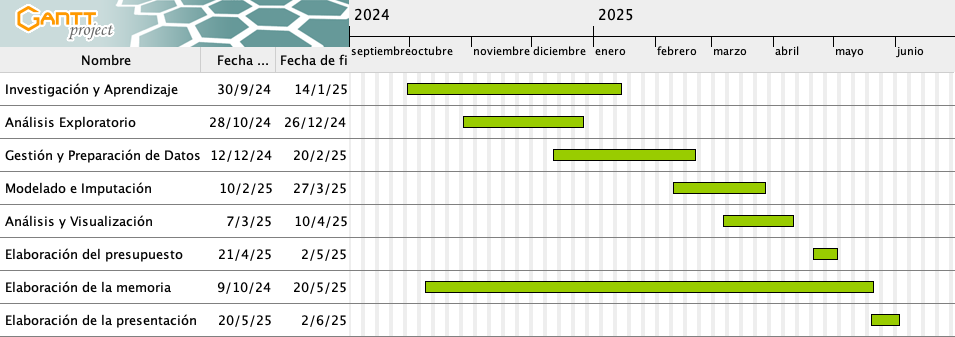
\includegraphics[width=0.9\textwidth]{images/planificacion.png} % Ajusta el width si es necesario
    \captionof{figure}{Diagrama de Gantt de la planificación inicial estimada para la realización del TFG.}
    \label{fig:gantt_planificacion}

    \vspace{1cm} % Espacio vertical entre las figuras (ajustar si es necesario)

    % Figura 2: Cronograma Real
    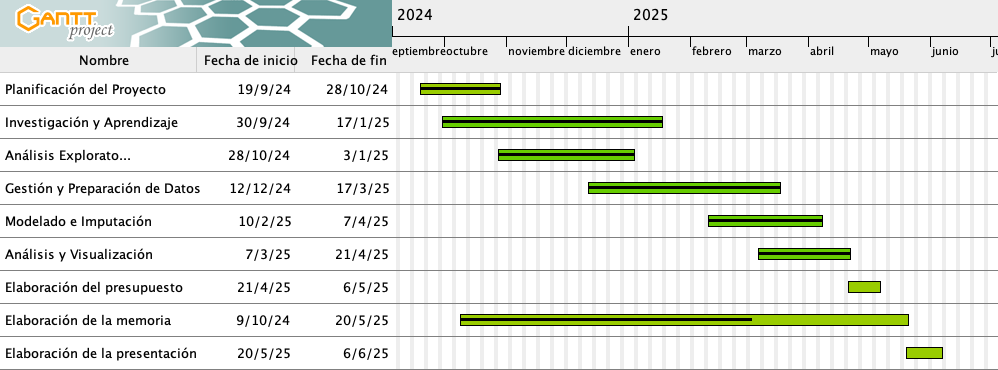
\includegraphics[width=0.9\textwidth]{images/cronograma.png} % Ajusta el width si es necesario
    \captionof{figure}{Diagrama de Gantt del progreso real durante la realización del TFG.}
    \label{fig:gantt_cronograma_real}

\end{figure}

La comparación entre ambos cronogramas evidencia que el desarrollo real del proyecto sufrió una desviación con respecto a la planificación inicial. Este retraso se debió principalmente a los siguientes factores:
\begin{itemize}
    \item \textbf{Profundización en el Estado del Arte:} La revisión bibliográfica y el estudio de trabajos previos requirieron más tiempo del previsto para establecer una base teórica robusta y contextualizar adecuadamente el proyecto.
    \item \textbf{Complejidad de la Arquitectura Transformer:} Comprender en detalle los mecanismos de atención y la implementación de los modelos Transformer supuso una inversión de tiempo considerable, fundamental para su correcta aplicación.
    \item \textbf{Curva de Aprendizaje de Bibliotecas:} La familiarización y el manejo eficiente de las bibliotecas de Python utilizadas (e.g., PyPOTS basada en PyTorch, Pandas, Numpy para manipulación de datos y Matplotlib para visualización) implicaron un periodo de adaptación necesario para la implementación práctica.
\end{itemize}


% --- Texto Presupuesto y Anexo B ---
\subsection*{Análisis del Presupuesto del Proyecto}

El presupuesto presentado a continuación se basa en la contabilización precisa de las horas dedicadas a cada tarea del TFG, registradas sistemáticamente con Timewarrior a lo largo de todo el desarrollo. Para la valoración económica, se ha aplicado una tarifa de 10 euros/hora.

Para facilitar la comprensión y el análisis del presupuesto, el trabajo registrado se ha clasificado en tres categorías principales, siguiendo una estructura habitual:
\begin{itemize}
    \item \textbf{Parte teórica:} Recoge las tareas relacionadas con el análisis conceptual, el estudio del estado del arte y la fundamentación teórica del proyecto. Corresponde a la categoría agrupada \textit{Investigación y Aprendizaje}.
    \item \textbf{Parte práctica:} Reúne las actividades directamente vinculadas con la implementación, programación, experimentación, análisis de datos y validación. Engloba las categorías de \textit{Pipeline y Datos}, \textit{Modelado y Entrenamiento}, \textit{Imputación y Nulos}, \textit{Análisis y Visualización}, y \textit{Metodología y Estructura}.
    \item \textbf{Parte general:} Agrupa las labores transversales de gestión del proyecto, comunicación (reuniones con tutores, correos), documentación y elaboración de la memoria. Corresponde a la categoría \textit{Gestión y Comunicaciones}.
\end{itemize}
Además de los costes derivados de las horas de trabajo, se incluye el coste amortizado del equipamiento principal utilizado (Macbook Air M2), considerando una vida útil estimada de 7 años. El desglose detallado del presupuesto se presenta en el \textbf{Anexo B} (Cuadro~\ref{tab:presupuesto_estimado}).

\newpage

\section*{Anexo B: Presupuesto Estimado}
\addcontentsline{toc}{section}{Anexo B: Presupuesto Estimado} % Añade este anexo a la TOC

\begin{table}[htbp]
    \centering
    \caption{Estimación del coste del proyecto basado en horas reales registradas.}
    \label{tab:presupuesto_estimado} % Label único y descriptivo
    % Definición de columnas: Izquierda, Número(Horas), Número(Tarifa), Número(Coste Total)
    \begin{tabular}{l S[table-format=3.1] S[table-format=2.0] S[table-format=4.2]}
        \toprule
        % Encabezados principales en negrita
        \textbf{Concepto} & {\textbf{Tiempo}} & {\textbf{Precio}} & {\textbf{Coste}} \\
        % Unidades/descripción bajo los encabezados, en cursiva y tamaño normal
         & {(\textit{horas})} & {(\textit{euros/hora})} & {(\textit{euros})} \\
        \midrule

        % --- Parte Teórica ---
        \multicolumn{4}{l}{\textbf{Parte general}} \\
        % Nombre completo de la categoría
        \quad Gestión y Comunicaciones & 1.4 & 10 & 14.00 \\ % Corrección: Las horas de I y A son 1.4
        \midrule

             % --- Parte General ---
        \multicolumn{4}{l}{\textbf{Parte teórica}} \\
        % Nombre completo de la categoría
        \quad Investigación y Aprendizaje  & 278.8 & 10 & 2788.00 \\ % Corrección: Las horas de G y C son 278.8
        \midrule


        % --- Parte Práctica ---
        \multicolumn{4}{l}{\textbf{Parte práctica}} \\
        % Nombres completos de las sub-categorías prácticas
        \quad Pipeline y Datos           & 43.6  & 10 & 436.00  \\
        \quad Modelado y Entrenamiento   & 40.6  & 10 & 406.00  \\
        \quad Imputación y Nulos         & 230.5 & 10 & 2305.00 \\
        \quad Análisis y Visualización   & 7.0   & 10 & 70.00   \\
        \quad Metodología y Estructura   & 4.4   & 10 & 44.00   \\
        \quad Equipo/Vida útil - Macbook Air M2 / 7 años    & {-}   & {-} & 162.70 \\
        \midrule

        % --- Cómputo Total ---
        % Subtotal Horas: 278.8 + 1.4 + 43.6 + 40.6 + 230.5 + 7.0 + 4.4 = 606.3
        % Subtotal Coste Horas: 2788.00 + 14.00 + 436.00 + 406.00 + 2305.00 + 70.00 + 44.00 = 6063.00
        % Coste Total: 6063.00 (Horas) + 162.70 (Equipo) = 6225.70
        \textbf{Coste total del proyecto} & \textbf{606.3} & {-} & \textbf{6225.70} \\
        \bottomrule
    \end{tabular}
    \par\medskip % Pequeño espacio después de la tabla (opcional)
    \footnotesize % Nota al pie más pequeña (opcional)
    \textit{Nota: Las horas reflejan el tiempo total registrado con Timewarrior para las tareas agrupadas en cada categoría. El coste del equipo representa una amortización estimada durante el periodo del proyecto.}
\end{table}
\clearpage % Opcional

% --- FIN CÓDIGO PARA anexos.tex ---

\chapter*{Anexos} % Título general para la sección de anexos (opcional)
\addcontentsline{toc}{chapter}{Anexos} % Añade la sección general a la TOC

% --- Texto Introductorio y Planificación ---
\section*{Planificación del Trabajo y Análisis del Presupuesto}
\label{sec:planificacion_presupuesto_intro} % Label para la sección

En esta sección se detalla tanto la planificación estimada inicial como la seguida durante el desarrollo del Trabajo Fin de Grado (TFG), junto con un análisis del presupuesto basado en el tiempo real invertido. La planificación y el seguimiento se visualizan a través de diagramas de Gantt generados con el software de código abierto \textbf{GanttProject}\footnote{\url{https://www.ganttproject.biz/}}. El análisis presupuestario se fundamenta en las \textbf{horas reales de trabajo registradas} mediante la herramienta de gestión de tiempo de código abierto \textbf{Timewarrior}\footnote{\url{https://timewarrior.net/}}. El objetivo es ofrecer una valoración transparente y fiel a la dedicación invertida en el proyecto, contrastando la planificación inicial con la ejecución real.

\subsection*{Planificación del Trabajo: Estimación vs. Realidad}

El diseño inicial y el posterior seguimiento de la planificación del proyecto se han gestionado utilizando GanttProject. En el \textbf{Anexo A} se presentan dos diagramas de Gantt para ilustrar la diferencia entre la estimación inicial y el progreso real:
\begin{itemize}
    \item La \textbf{Figura~\ref{fig:gantt_planificacion}} muestra una planificación inicial optimista, elaborada al comienzo del proyecto.
    \item La \textbf{Figura~\ref{fig:gantt_cronograma_real}} refleja la progresión y duración real de las tareas, tal como se desarrollaron.
\end{itemize}

\newpage
% --- ANEXO A: CRONOGRAMAS ---
\section*{Anexo A: Cronogramas}
\addcontentsline{toc}{section}{Anexo A: Cronogramas} % Añade este anexo a la TOC

\begin{figure}[htbp] % Entorno para ambas figuras
    \centering % Centrar ambas figuras

    % Figura 1: Planificación Inicial
    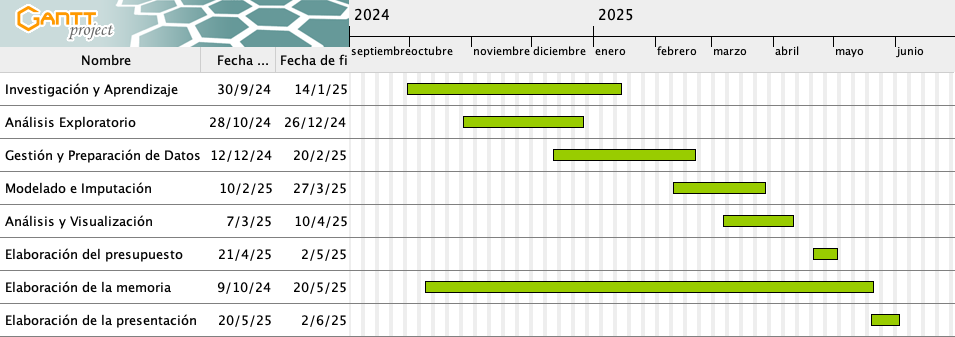
\includegraphics[width=0.9\textwidth]{images/planificacion.png} % Ajusta el width si es necesario
    \captionof{figure}{Diagrama de Gantt de la planificación inicial estimada para la realización del TFG.}
    \label{fig:gantt_planificacion}

    \vspace{1cm} % Espacio vertical entre las figuras (ajustar si es necesario)

    % Figura 2: Cronograma Real
    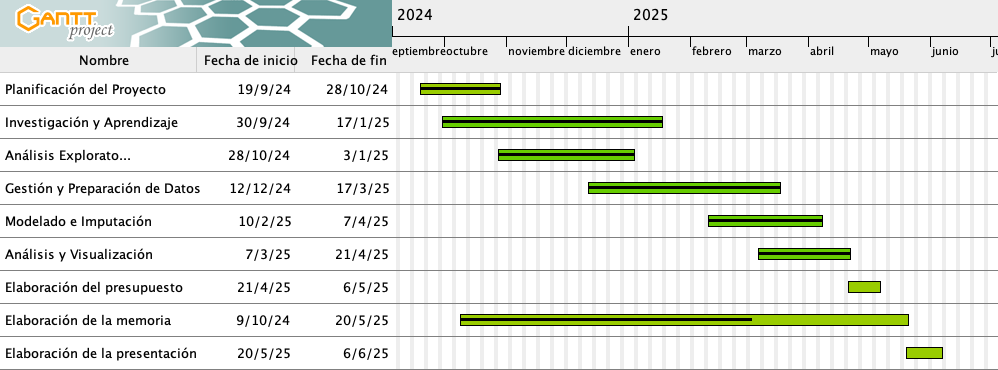
\includegraphics[width=0.9\textwidth]{images/cronograma.png} % Ajusta el width si es necesario
    \captionof{figure}{Diagrama de Gantt del progreso real durante la realización del TFG.}
    \label{fig:gantt_cronograma_real}

\end{figure}

La comparación entre ambos cronogramas evidencia que el desarrollo real del proyecto sufrió una desviación con respecto a la planificación inicial. Este retraso se debió principalmente a los siguientes factores:
\begin{itemize}
    \item \textbf{Profundización en el Estado del Arte:} La revisión bibliográfica y el estudio de trabajos previos requirieron más tiempo del previsto para establecer una base teórica robusta y contextualizar adecuadamente el proyecto.
    \item \textbf{Complejidad de la Arquitectura Transformer:} Comprender en detalle los mecanismos de atención y la implementación de los modelos Transformer supuso una inversión de tiempo considerable, fundamental para su correcta aplicación.
    \item \textbf{Curva de Aprendizaje de Bibliotecas:} La familiarización y el manejo eficiente de las bibliotecas de Python utilizadas (e.g., PyPOTS basada en PyTorch, Pandas, Numpy para manipulación de datos y Matplotlib para visualización) implicaron un periodo de adaptación necesario para la implementación práctica.
\end{itemize}


% --- Texto Presupuesto y Anexo B ---
\subsection*{Análisis del Presupuesto del Proyecto}

El presupuesto presentado a continuación se basa en la contabilización precisa de las horas dedicadas a cada tarea del TFG, registradas sistemáticamente con Timewarrior a lo largo de todo el desarrollo. Para la valoración económica, se ha aplicado una tarifa de 10 euros/hora.

Para facilitar la comprensión y el análisis del presupuesto, el trabajo registrado se ha clasificado en tres categorías principales, siguiendo una estructura habitual:
\begin{itemize}
    \item \textbf{Parte teórica:} Recoge las tareas relacionadas con el análisis conceptual, el estudio del estado del arte y la fundamentación teórica del proyecto. Corresponde a la categoría agrupada \textit{Investigación y Aprendizaje}.
    \item \textbf{Parte práctica:} Reúne las actividades directamente vinculadas con la implementación, programación, experimentación, análisis de datos y validación. Engloba las categorías de \textit{Pipeline y Datos}, \textit{Modelado y Entrenamiento}, \textit{Imputación y Nulos}, \textit{Análisis y Visualización}, y \textit{Metodología y Estructura}.
    \item \textbf{Parte general:} Agrupa las labores transversales de gestión del proyecto, comunicación (reuniones con tutores, correos), documentación y elaboración de la memoria. Corresponde a la categoría \textit{Gestión y Comunicaciones}.
\end{itemize}
Además de los costes derivados de las horas de trabajo, se incluye el coste amortizado del equipamiento principal utilizado (Macbook Air M2), considerando una vida útil estimada de 7 años. El desglose detallado del presupuesto se presenta en el \textbf{Anexo B} (Cuadro~\ref{tab:presupuesto_estimado}).

\newpage

\section*{Anexo B: Presupuesto Estimado}
\addcontentsline{toc}{section}{Anexo B: Presupuesto Estimado} % Añade este anexo a la TOC

\begin{table}[htbp]
    \centering
    \caption{Estimación del coste del proyecto basado en horas reales registradas.}
    \label{tab:presupuesto_estimado} % Label único y descriptivo
    % Definición de columnas: Izquierda, Número(Horas), Número(Tarifa), Número(Coste Total)
    \begin{tabular}{l S[table-format=3.1] S[table-format=2.0] S[table-format=4.2]}
        \toprule
        % Encabezados principales en negrita
        \textbf{Concepto} & {\textbf{Tiempo}} & {\textbf{Precio}} & {\textbf{Coste}} \\
        % Unidades/descripción bajo los encabezados, en cursiva y tamaño normal
         & {(\textit{horas})} & {(\textit{euros/hora})} & {(\textit{euros})} \\
        \midrule

        % --- Parte Teórica ---
        \multicolumn{4}{l}{\textbf{Parte general}} \\
        % Nombre completo de la categoría
        \quad Gestión y Comunicaciones & 1.4 & 10 & 14.00 \\ % Corrección: Las horas de I y A son 1.4
        \midrule

             % --- Parte General ---
        \multicolumn{4}{l}{\textbf{Parte teórica}} \\
        % Nombre completo de la categoría
        \quad Investigación y Aprendizaje  & 278.8 & 10 & 2788.00 \\ % Corrección: Las horas de G y C son 278.8
        \midrule


        % --- Parte Práctica ---
        \multicolumn{4}{l}{\textbf{Parte práctica}} \\
        % Nombres completos de las sub-categorías prácticas
        \quad Pipeline y Datos           & 43.6  & 10 & 436.00  \\
        \quad Modelado y Entrenamiento   & 40.6  & 10 & 406.00  \\
        \quad Imputación y Nulos         & 230.5 & 10 & 2305.00 \\
        \quad Análisis y Visualización   & 7.0   & 10 & 70.00   \\
        \quad Metodología y Estructura   & 4.4   & 10 & 44.00   \\
        \quad Equipo/Vida útil - Macbook Air M2 / 7 años    & {-}   & {-} & 162.70 \\
        \midrule

        % --- Cómputo Total ---
        % Subtotal Horas: 278.8 + 1.4 + 43.6 + 40.6 + 230.5 + 7.0 + 4.4 = 606.3
        % Subtotal Coste Horas: 2788.00 + 14.00 + 436.00 + 406.00 + 2305.00 + 70.00 + 44.00 = 6063.00
        % Coste Total: 6063.00 (Horas) + 162.70 (Equipo) = 6225.70
        \textbf{Coste total del proyecto} & \textbf{606.3} & {-} & \textbf{6225.70} \\
        \bottomrule
    \end{tabular}
    \par\medskip % Pequeño espacio después de la tabla (opcional)
    \footnotesize % Nota al pie más pequeña (opcional)
    \textit{Nota: Las horas reflejan el tiempo total registrado con Timewarrior para las tareas agrupadas en cada categoría. El coste del equipo representa una amortización estimada durante el periodo del proyecto.}
\end{table}
\clearpage % Opcional

% --- FIN CÓDIGO PARA anexos.tex ---

\chapter*{Anexos} % Título general para la sección de anexos (opcional)
\addcontentsline{toc}{chapter}{Anexos} % Añade la sección general a la TOC

% --- Texto Introductorio y Planificación ---
\section*{Planificación del Trabajo y Análisis del Presupuesto}
\label{sec:planificacion_presupuesto_intro} % Label para la sección

En esta sección se detalla tanto la planificación estimada inicial como la seguida durante el desarrollo del Trabajo Fin de Grado (TFG), junto con un análisis del presupuesto basado en el tiempo real invertido. La planificación y el seguimiento se visualizan a través de diagramas de Gantt generados con el software de código abierto \textbf{GanttProject}\footnote{\url{https://www.ganttproject.biz/}}. El análisis presupuestario se fundamenta en las \textbf{horas reales de trabajo registradas} mediante la herramienta de gestión de tiempo de código abierto \textbf{Timewarrior}\footnote{\url{https://timewarrior.net/}}. El objetivo es ofrecer una valoración transparente y fiel a la dedicación invertida en el proyecto, contrastando la planificación inicial con la ejecución real.

\subsection*{Planificación del Trabajo: Estimación vs. Realidad}

El diseño inicial y el posterior seguimiento de la planificación del proyecto se han gestionado utilizando GanttProject. En el \textbf{Anexo A} se presentan dos diagramas de Gantt para ilustrar la diferencia entre la estimación inicial y el progreso real:
\begin{itemize}
    \item La \textbf{Figura~\ref{fig:gantt_planificacion}} muestra una planificación inicial optimista, elaborada al comienzo del proyecto.
    \item La \textbf{Figura~\ref{fig:gantt_cronograma_real}} refleja la progresión y duración real de las tareas, tal como se desarrollaron.
\end{itemize}

\newpage
% --- ANEXO A: CRONOGRAMAS ---
\section*{Anexo A: Cronogramas}
\addcontentsline{toc}{section}{Anexo A: Cronogramas} % Añade este anexo a la TOC

\begin{figure}[htbp] % Entorno para ambas figuras
    \centering % Centrar ambas figuras

    % Figura 1: Planificación Inicial
    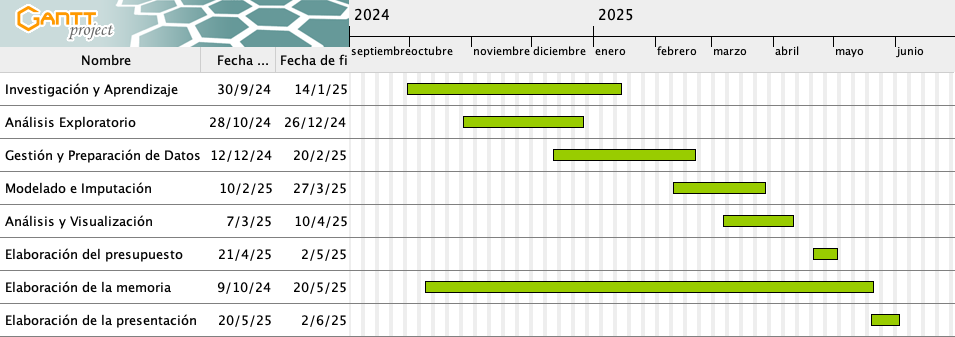
\includegraphics[width=0.9\textwidth]{images/planificacion.png} % Ajusta el width si es necesario
    \captionof{figure}{Diagrama de Gantt de la planificación inicial estimada para la realización del TFG.}
    \label{fig:gantt_planificacion}

    \vspace{1cm} % Espacio vertical entre las figuras (ajustar si es necesario)

    % Figura 2: Cronograma Real
    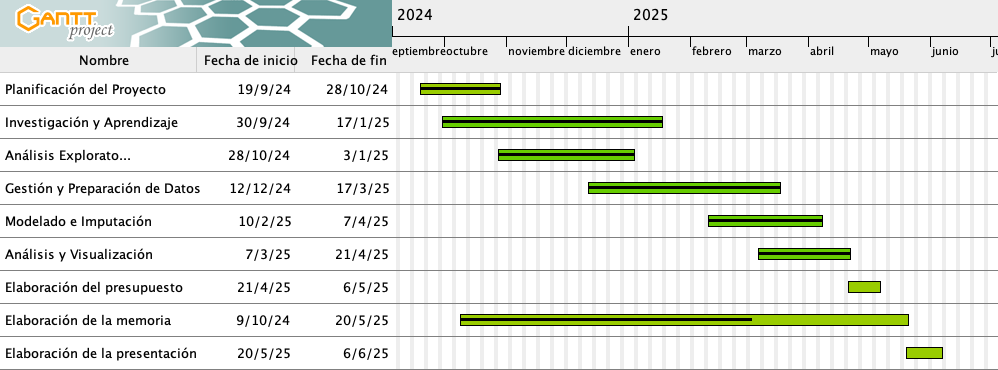
\includegraphics[width=0.9\textwidth]{images/cronograma.png} % Ajusta el width si es necesario
    \captionof{figure}{Diagrama de Gantt del progreso real durante la realización del TFG.}
    \label{fig:gantt_cronograma_real}

\end{figure}

La comparación entre ambos cronogramas evidencia que el desarrollo real del proyecto sufrió una desviación con respecto a la planificación inicial. Este retraso se debió principalmente a los siguientes factores:
\begin{itemize}
    \item \textbf{Profundización en el Estado del Arte:} La revisión bibliográfica y el estudio de trabajos previos requirieron más tiempo del previsto para establecer una base teórica robusta y contextualizar adecuadamente el proyecto.
    \item \textbf{Complejidad de la Arquitectura Transformer:} Comprender en detalle los mecanismos de atención y la implementación de los modelos Transformer supuso una inversión de tiempo considerable, fundamental para su correcta aplicación.
    \item \textbf{Curva de Aprendizaje de Bibliotecas:} La familiarización y el manejo eficiente de las bibliotecas de Python utilizadas (e.g., PyPOTS basada en PyTorch, Pandas, Numpy para manipulación de datos y Matplotlib para visualización) implicaron un periodo de adaptación necesario para la implementación práctica.
\end{itemize}


% --- Texto Presupuesto y Anexo B ---
\subsection*{Análisis del Presupuesto del Proyecto}

El presupuesto presentado a continuación se basa en la contabilización precisa de las horas dedicadas a cada tarea del TFG, registradas sistemáticamente con Timewarrior a lo largo de todo el desarrollo. Para la valoración económica, se ha aplicado una tarifa de 10 euros/hora.

Para facilitar la comprensión y el análisis del presupuesto, el trabajo registrado se ha clasificado en tres categorías principales, siguiendo una estructura habitual:
\begin{itemize}
    \item \textbf{Parte teórica:} Recoge las tareas relacionadas con el análisis conceptual, el estudio del estado del arte y la fundamentación teórica del proyecto. Corresponde a la categoría agrupada \textit{Investigación y Aprendizaje}.
    \item \textbf{Parte práctica:} Reúne las actividades directamente vinculadas con la implementación, programación, experimentación, análisis de datos y validación. Engloba las categorías de \textit{Pipeline y Datos}, \textit{Modelado y Entrenamiento}, \textit{Imputación y Nulos}, \textit{Análisis y Visualización}, y \textit{Metodología y Estructura}.
    \item \textbf{Parte general:} Agrupa las labores transversales de gestión del proyecto, comunicación (reuniones con tutores, correos), documentación y elaboración de la memoria. Corresponde a la categoría \textit{Gestión y Comunicaciones}.
\end{itemize}
Además de los costes derivados de las horas de trabajo, se incluye el coste amortizado del equipamiento principal utilizado (Macbook Air M2), considerando una vida útil estimada de 7 años. El desglose detallado del presupuesto se presenta en el \textbf{Anexo B} (Cuadro~\ref{tab:presupuesto_estimado}).

\newpage

\section*{Anexo B: Presupuesto Estimado}
\addcontentsline{toc}{section}{Anexo B: Presupuesto Estimado} % Añade este anexo a la TOC

\begin{table}[htbp]
    \centering
    \caption{Estimación del coste del proyecto basado en horas reales registradas.}
    \label{tab:presupuesto_estimado} % Label único y descriptivo
    % Definición de columnas: Izquierda, Número(Horas), Número(Tarifa), Número(Coste Total)
    \begin{tabular}{l S[table-format=3.1] S[table-format=2.0] S[table-format=4.2]}
        \toprule
        % Encabezados principales en negrita
        \textbf{Concepto} & {\textbf{Tiempo}} & {\textbf{Precio}} & {\textbf{Coste}} \\
        % Unidades/descripción bajo los encabezados, en cursiva y tamaño normal
         & {(\textit{horas})} & {(\textit{euros/hora})} & {(\textit{euros})} \\
        \midrule

        % --- Parte Teórica ---
        \multicolumn{4}{l}{\textbf{Parte general}} \\
        % Nombre completo de la categoría
        \quad Gestión y Comunicaciones & 1.4 & 10 & 14.00 \\ % Corrección: Las horas de I y A son 1.4
        \midrule

             % --- Parte General ---
        \multicolumn{4}{l}{\textbf{Parte teórica}} \\
        % Nombre completo de la categoría
        \quad Investigación y Aprendizaje  & 278.8 & 10 & 2788.00 \\ % Corrección: Las horas de G y C son 278.8
        \midrule


        % --- Parte Práctica ---
        \multicolumn{4}{l}{\textbf{Parte práctica}} \\
        % Nombres completos de las sub-categorías prácticas
        \quad Pipeline y Datos           & 43.6  & 10 & 436.00  \\
        \quad Modelado y Entrenamiento   & 40.6  & 10 & 406.00  \\
        \quad Imputación y Nulos         & 230.5 & 10 & 2305.00 \\
        \quad Análisis y Visualización   & 7.0   & 10 & 70.00   \\
        \quad Metodología y Estructura   & 4.4   & 10 & 44.00   \\
        \quad Equipo/Vida útil - Macbook Air M2 / 7 años    & {-}   & {-} & 162.70 \\
        \midrule

        % --- Cómputo Total ---
        % Subtotal Horas: 278.8 + 1.4 + 43.6 + 40.6 + 230.5 + 7.0 + 4.4 = 606.3
        % Subtotal Coste Horas: 2788.00 + 14.00 + 436.00 + 406.00 + 2305.00 + 70.00 + 44.00 = 6063.00
        % Coste Total: 6063.00 (Horas) + 162.70 (Equipo) = 6225.70
        \textbf{Coste total del proyecto} & \textbf{606.3} & {-} & \textbf{6225.70} \\
        \bottomrule
    \end{tabular}
    \par\medskip % Pequeño espacio después de la tabla (opcional)
    \footnotesize % Nota al pie más pequeña (opcional)
    \textit{Nota: Las horas reflejan el tiempo total registrado con Timewarrior para las tareas agrupadas en cada categoría. El coste del equipo representa una amortización estimada durante el periodo del proyecto.}
\end{table}
\clearpage % Opcional

% --- FIN CÓDIGO PARA anexos.tex ---

\chapter*{Anexos} % Título general para la sección de anexos (opcional)
\addcontentsline{toc}{chapter}{Anexos} % Añade la sección general a la TOC

% --- Texto Introductorio y Planificación ---
\section*{Planificación del Trabajo y Análisis del Presupuesto}
\label{sec:planificacion_presupuesto_intro} % Label para la sección

En esta sección se detalla tanto la planificación estimada inicial como la seguida durante el desarrollo del Trabajo Fin de Grado (TFG), junto con un análisis del presupuesto basado en el tiempo real invertido. La planificación y el seguimiento se visualizan a través de diagramas de Gantt generados con el software de código abierto \textbf{GanttProject}\footnote{\url{https://www.ganttproject.biz/}}. El análisis presupuestario se fundamenta en las \textbf{horas reales de trabajo registradas} mediante la herramienta de gestión de tiempo de código abierto \textbf{Timewarrior}\footnote{\url{https://timewarrior.net/}}. El objetivo es ofrecer una valoración transparente y fiel a la dedicación invertida en el proyecto, contrastando la planificación inicial con la ejecución real.

\subsection*{Planificación del Trabajo: Estimación vs. Realidad}

El diseño inicial y el posterior seguimiento de la planificación del proyecto se han gestionado utilizando GanttProject. En el \textbf{Anexo A} se presentan dos diagramas de Gantt para ilustrar la diferencia entre la estimación inicial y el progreso real:
\begin{itemize}
    \item La \textbf{Figura~\ref{fig:gantt_planificacion}} muestra una planificación inicial optimista, elaborada al comienzo del proyecto.
    \item La \textbf{Figura~\ref{fig:gantt_cronograma_real}} refleja la progresión y duración real de las tareas, tal como se desarrollaron.
\end{itemize}

\newpage
% --- ANEXO A: CRONOGRAMAS ---
\section*{Anexo A: Cronogramas}
\addcontentsline{toc}{section}{Anexo A: Cronogramas} % Añade este anexo a la TOC

\begin{figure}[htbp] % Entorno para ambas figuras
    \centering % Centrar ambas figuras

    % Figura 1: Planificación Inicial
    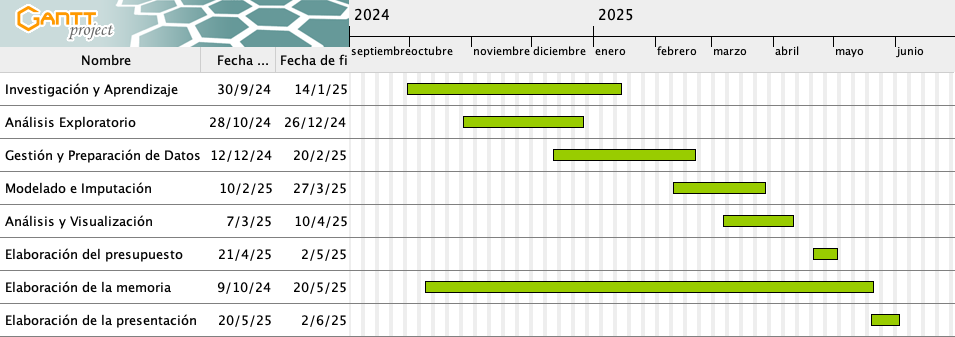
\includegraphics[width=0.9\textwidth]{images/planificacion.png} % Ajusta el width si es necesario
    \captionof{figure}{Diagrama de Gantt de la planificación inicial estimada para la realización del TFG.}
    \label{fig:gantt_planificacion}

    \vspace{1cm} % Espacio vertical entre las figuras (ajustar si es necesario)

    % Figura 2: Cronograma Real
    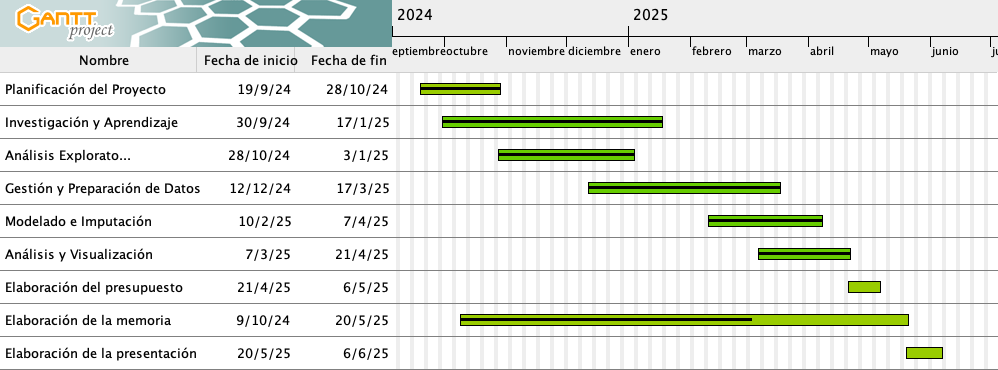
\includegraphics[width=0.9\textwidth]{images/cronograma.png} % Ajusta el width si es necesario
    \captionof{figure}{Diagrama de Gantt del progreso real durante la realización del TFG.}
    \label{fig:gantt_cronograma_real}

\end{figure}

La comparación entre ambos cronogramas evidencia que el desarrollo real del proyecto sufrió una desviación con respecto a la planificación inicial. Este retraso se debió principalmente a los siguientes factores:
\begin{itemize}
    \item \textbf{Profundización en el Estado del Arte:} La revisión bibliográfica y el estudio de trabajos previos requirieron más tiempo del previsto para establecer una base teórica robusta y contextualizar adecuadamente el proyecto.
    \item \textbf{Complejidad de la Arquitectura Transformer:} Comprender en detalle los mecanismos de atención y la implementación de los modelos Transformer supuso una inversión de tiempo considerable, fundamental para su correcta aplicación.
    \item \textbf{Curva de Aprendizaje de Bibliotecas:} La familiarización y el manejo eficiente de las bibliotecas de Python utilizadas (e.g., PyPOTS basada en PyTorch, Pandas, Numpy para manipulación de datos y Matplotlib para visualización) implicaron un periodo de adaptación necesario para la implementación práctica.
\end{itemize}


% --- Texto Presupuesto y Anexo B ---
\subsection*{Análisis del Presupuesto del Proyecto}

El presupuesto presentado a continuación se basa en la contabilización precisa de las horas dedicadas a cada tarea del TFG, registradas sistemáticamente con Timewarrior a lo largo de todo el desarrollo. Para la valoración económica, se ha aplicado una tarifa de 10 euros/hora.

Para facilitar la comprensión y el análisis del presupuesto, el trabajo registrado se ha clasificado en tres categorías principales, siguiendo una estructura habitual:
\begin{itemize}
    \item \textbf{Parte teórica:} Recoge las tareas relacionadas con el análisis conceptual, el estudio del estado del arte y la fundamentación teórica del proyecto. Corresponde a la categoría agrupada \textit{Investigación y Aprendizaje}.
    \item \textbf{Parte práctica:} Reúne las actividades directamente vinculadas con la implementación, programación, experimentación, análisis de datos y validación. Engloba las categorías de \textit{Pipeline y Datos}, \textit{Modelado y Entrenamiento}, \textit{Imputación y Nulos}, \textit{Análisis y Visualización}, y \textit{Metodología y Estructura}.
    \item \textbf{Parte general:} Agrupa las labores transversales de gestión del proyecto, comunicación (reuniones con tutores, correos), documentación y elaboración de la memoria. Corresponde a la categoría \textit{Gestión y Comunicaciones}.
\end{itemize}
Además de los costes derivados de las horas de trabajo, se incluye el coste amortizado del equipamiento principal utilizado (Macbook Air M2), considerando una vida útil estimada de 7 años. El desglose detallado del presupuesto se presenta en el \textbf{Anexo B} (Cuadro~\ref{tab:presupuesto_estimado}).

\newpage

\section*{Anexo B: Presupuesto Estimado}
\addcontentsline{toc}{section}{Anexo B: Presupuesto Estimado} % Añade este anexo a la TOC

\begin{table}[htbp]
    \centering
    \caption{Estimación del coste del proyecto basado en horas reales registradas.}
    \label{tab:presupuesto_estimado} % Label único y descriptivo
    % Definición de columnas: Izquierda, Número(Horas), Número(Tarifa), Número(Coste Total)
    \begin{tabular}{l S[table-format=3.1] S[table-format=2.0] S[table-format=4.2]}
        \toprule
        % Encabezados principales en negrita
        \textbf{Concepto} & {\textbf{Tiempo}} & {\textbf{Precio}} & {\textbf{Coste}} \\
        % Unidades/descripción bajo los encabezados, en cursiva y tamaño normal
         & {(\textit{horas})} & {(\textit{euros/hora})} & {(\textit{euros})} \\
        \midrule

        % --- Parte Teórica ---
        \multicolumn{4}{l}{\textbf{Parte general}} \\
        % Nombre completo de la categoría
        \quad Gestión y Comunicaciones & 1.4 & 10 & 14.00 \\ % Corrección: Las horas de I y A son 1.4
        \midrule

             % --- Parte General ---
        \multicolumn{4}{l}{\textbf{Parte teórica}} \\
        % Nombre completo de la categoría
        \quad Investigación y Aprendizaje  & 278.8 & 10 & 2788.00 \\ % Corrección: Las horas de G y C son 278.8
        \midrule


        % --- Parte Práctica ---
        \multicolumn{4}{l}{\textbf{Parte práctica}} \\
        % Nombres completos de las sub-categorías prácticas
        \quad Pipeline y Datos           & 43.6  & 10 & 436.00  \\
        \quad Modelado y Entrenamiento   & 40.6  & 10 & 406.00  \\
        \quad Imputación y Nulos         & 230.5 & 10 & 2305.00 \\
        \quad Análisis y Visualización   & 7.0   & 10 & 70.00   \\
        \quad Metodología y Estructura   & 4.4   & 10 & 44.00   \\
        \quad Equipo/Vida útil - Macbook Air M2 / 7 años    & {-}   & {-} & 162.70 \\
        \midrule

        % --- Cómputo Total ---
        % Subtotal Horas: 278.8 + 1.4 + 43.6 + 40.6 + 230.5 + 7.0 + 4.4 = 606.3
        % Subtotal Coste Horas: 2788.00 + 14.00 + 436.00 + 406.00 + 2305.00 + 70.00 + 44.00 = 6063.00
        % Coste Total: 6063.00 (Horas) + 162.70 (Equipo) = 6225.70
        \textbf{Coste total del proyecto} & \textbf{606.3} & {-} & \textbf{6225.70} \\
        \bottomrule
    \end{tabular}
    \par\medskip % Pequeño espacio después de la tabla (opcional)
    \footnotesize % Nota al pie más pequeña (opcional)
    \textit{Nota: Las horas reflejan el tiempo total registrado con Timewarrior para las tareas agrupadas en cada categoría. El coste del equipo representa una amortización estimada durante el periodo del proyecto.}
\end{table}
\clearpage % Opcional

% --- FIN CÓDIGO PARA anexos.tex ---